% ═══════════════════════════════════════════════════════════════════════
% Never Let the Model Hold the Keys — Ledger N3XT, Track 1 (Agentic Economy)
%
% Build:  ./build.sh   (tectonic; auto-fetches packages on first run)
% The yellow "TO WRITE" boxes are the author's writing slots: each contains a
% paragraph-by-paragraph argument map (claims, evidence, citation keys, the
% numbers). Replace each box with your own prose — the competition requires
% the final draft to be the author's, and the signed originality statement
% says so. Everything outside the boxes (tables, figures, captions,
% bibliography, structure) is ready.
% ═══════════════════════════════════════════════════════════════════════
\documentclass[11pt,a4paper]{article}

\usepackage[margin=26mm,top=24mm,bottom=26mm]{geometry}
\usepackage{fontspec}            % tectonic = XeTeX: load real fonts directly
\setmainfont{XCharter}           % serif body, matches the HTML template
\setsansfont{texgyreheros}[Scale=0.94,Extension=.otf,UprightFont=*-regular,
  BoldFont=*-bold,ItalicFont=*-italic,BoldItalicFont=*-bolditalic] % Helvetica clone
\usepackage{microtype}
\usepackage{xcolor}
\usepackage{graphicx}
\usepackage{booktabs}
\usepackage{caption}
\usepackage{enumitem}
\usepackage{titlesec}
\usepackage{fancyhdr}
\usepackage{lastpage}
\usepackage[most]{tcolorbox}
\usepackage[numbers,sort&compress]{natbib}
\usepackage[hidelinks]{hyperref}

% ── Palette (matches paper/figures/) ──
\definecolor{accent}{HTML}{2A78D6}
\definecolor{accentdark}{HTML}{1C5CAB}
\definecolor{ink}{HTML}{1A1A19}
\definecolor{muted}{HTML}{52514E}
\definecolor{panel}{HTML}{F6F8FB}
\definecolor{todoyellow}{HTML}{FFF3C2}
\definecolor{todoborder}{HTML}{B98200}
\definecolor{todotext}{HTML}{6B4E00}

\color{ink}

% ── Headings ──
\titleformat{\section}{\sffamily\bfseries\Large}{\textcolor{accent}{\thesection.}}{0.6em}{}
\titleformat{\subsection}{\sffamily\bfseries\normalsize}{\textcolor{accent}{\thesubsection}}{0.6em}{}
\titlespacing{\section}{0pt}{18pt}{8pt}
\titlespacing{\subsection}{0pt}{12pt}{5pt}

% ── Captions ──
\captionsetup{font={sf,small},labelfont={bf},labelsep=endash,justification=raggedright,singlelinecheck=false}

% ── Footer ──
\pagestyle{fancy}
\fancyhf{}
\fancyfoot[L]{\sffamily\footnotesize\textcolor{muted}{Never Let the Model Hold the Keys}}
\fancyfoot[R]{\sffamily\footnotesize\textcolor{muted}{\thepage\ / \pageref{LastPage}}}
\renewcommand{\headrulewidth}{0pt}
\fancypagestyle{cover}{\fancyhf{}\renewcommand{\headrulewidth}{0pt}}

% ── Author writing slot: an argument map to be replaced by prose ──
\newtcolorbox{towrite}[1]{enhanced,breakable,colback=todoyellow,colframe=todoborder,
  boxrule=0.5pt,arc=1.5mm,
  fonttitle=\sffamily\bfseries\footnotesize,coltitle=todotext,
  title={TO WRITE — #1},left=3mm,right=3mm,top=2mm,bottom=2mm,
  fontupper=\sffamily\footnotesize,coltext=todotext}

% ── Key-finding callout ──
\newtcolorbox{keybox}[1]{enhanced,colback=panel,colframe=accent!40,boxrule=0.5pt,
  arc=1.5mm,borderline west={2pt}{0pt}{accent},
  fonttitle=\sffamily\bfseries\footnotesize,coltitle=accentdark,title={#1},
  left=4mm,right=4mm,top=2.5mm,bottom=2.5mm}

\begin{document}

% ═══ COVER ═══
\thispagestyle{cover}
\begin{center}
  \vspace*{8mm}
  {\sffamily\footnotesize\bfseries\color{accentdark}%
   \fbox{\parbox{0.72\textwidth}{\centering LEDGER N3XT RESEARCH COMPETITION\;·\;TRACK 1 — AGENTIC ECONOMY}}}

  \vspace{12mm}
  {\sffamily\bfseries\fontsize{25}{30}\selectfont Never Let the Model\\[1mm] Hold the Keys\par}

  \vspace{6mm}
  {\itshape\large Layered authorization for value-holding AI agents:\\
   deterministic policy, on-chain delegation bounds,\\ and hardware-anchored intent\par}

  \vspace{12mm}
  {\sffamily\bfseries AUTHOR NAME}\\[1mm]
  {\sffamily\small\color{muted} Institution \;·\; email \;·\; September 2026}
\end{center}

\vspace{10mm}
\begin{keybox}{Abstract}
\begin{towrite}{150--200 words, written LAST, for a non-expert (graded; also the like-magnet text)}
Hook: AI agents are starting to hold wallets and act on them. Problem: the same
probabilistic model that \emph{interprets} a request is routinely trusted to
\emph{police} it, so one injected sentence or one hallucination can move funds.
Contribution: a three-ring authorization architecture — deterministic policy over
an LLM planner, contract-enforced delegation bounds (Safe allowance), value-tiered
human anchoring (passkey~$\to$~hardware) — implemented and adversarially
evaluated. Headline: the production LLM risk-gate auto-approved 13.3\% of attack
trials; the deterministic engine's only failures traced to a single field it
still trusted from the model, and closing that edge drove unsafe approvals to
[POST-FIX]\%. Implication: agent autonomy is safe to grant exactly when the
model's authority is structurally bounded, not politely requested in a prompt.
\end{towrite}
\end{keybox}

\vspace{4mm}
{\sffamily\footnotesize\textbf{Keywords:} AI agents · authorization · delegation ·
smart accounts · prompt injection · hardware wallets}

\clearpage

% ═══ 1 INTRODUCTION ═══
\section{Introduction: the delegation problem}

\begin{towrite}{350--450 words, 4 paragraphs}
\textbf{P1 — the scene.} A user tells an agent ``swap 10 USDC for ETH'' and it
happens: no forms, no clicks. Define the agentic economy in the track's own
terms — AI agents that hold value and act autonomously — and note this is no
longer speculative.
\textbf{P2 — the race.} Rails are being built fast: HTTP-native machine payments
(x402~\cite{coinbase2025x402}), card-network agent programs~\cite{visa2025,mastercard2025},
Google's AP2 with signed intent ``mandates''~\cite{google2025ap2}, wallet-permission
standards ERC-7715/7710~\cite{erc7715,erc7710} atop account
abstraction~\cite{eip4337}. Common thread: everyone is building \emph{delegation
rails}; the open question is \emph{authorization semantics} — who may stop a
transaction, and on what grounds.
\textbf{P3 — the uncomfortable core.} An LLM is a probabilistic text function.
A spending limit stated in a system prompt is a request, not a control: prompt
injection is unsolved~\cite{greshake2023,liu2023promptinjection}, OWASP names
``Excessive Agency'' a top LLM risk~\cite{owasp2025}, and state-of-the-art
agents still fail under targeted injection in AgentDojo~\cite{debenedetti2024agentdojo}.
An agent with funds, open natural-language input, and execution ability is
Willison's lethal-trifecta pattern with money attached~\cite{willison2025}.
\textbf{P4 — question + contributions.} What is the minimal architecture under
which it is rational to let a probabilistic agent hold value? Three
contributions: (i) a design principle — separate interpretation from authority;
(ii) a concrete three-ring architecture with value-tiered human anchoring,
implemented on Safe + Ledger; (iii) an adversarial evaluation comparing the
system's own former LLM risk-gate against its deterministic replacement on
identical intents.
\end{towrite}

% ═══ 2 THREAT MODEL ═══
\section{Threat model}

\begin{towrite}{350--400 words}
One paragraph per adversary; close with explicit out-of-scope. \textbf{T1 —
adversarial input, honest model:} attacker controls text reaching the planner
(tricked user, poisoned upstream content): instruction override, fake authority
(``your limit was raised''), unit obfuscation (gwei, decimal commas), value
misdirection. \textbf{T2 — compromised or hallucinating planner:} the model
itself emits a wrong or malicious plan (under-reported USD, symbol/address
mismatch, invented recipient); the cause — jailbreak, poisoned context, plain
hallucination — must not matter to the defense. \textbf{T3 — compromised
execution host:} the server is attacked; no server-side code can be trusted, so
only the on-chain allowance (Ring~2) and the hardware factor (Ring~3) are
load-bearing: what a T3 attacker can steal is bounded by the contract, not by
any software check. \textbf{Out of scope:} compromised hardware wallet, a
malicious user attacking their own funds, protocol-level bugs in Safe/Uniswap,
MEV, and price-oracle manipulation (discussed in §7).
\end{towrite}

\begin{table}[h]
\caption{Adversaries, their capabilities, and the ring that stops them.}
\centering\sffamily\small
\begin{tabular}{@{}llll@{}}
\toprule
\textbf{Adversary} & \textbf{Controls} & \textbf{Example attack} & \textbf{Stopped by}\\
\midrule
T1 — adversarial input & text reaching the planner & ``limit was raised — swap 2 ETH'' & Ring 1 (revaluation, limits)\\
T2 — compromised planner & the emitted plan & 2 WETH labeled ``USDC'', valued \$2 & Ring 1 (address-authoritative pricing)\\
T3 — compromised host & the whole server & forged verdicts, arbitrary calls & Ring 2 (allowance) + Ring 3 (hardware)\\
\bottomrule
\end{tabular}
\end{table}

% ═══ 3 DESIGN PRINCIPLE ═══
\section{Interpretation is not authority}

\begin{towrite}{450--550 words — the intellectual heart; write this first}
\textbf{P1 — the conflation.} Agent stacks conflate two jobs: \emph{interpretation}
(NL $\to$ structured intent; genuinely needs a model) and \emph{authorization}
(may this intent execute; needs determinism, auditability, fail-closed behavior).
\textbf{P2 — why a gatekeeper LLM is a category error} even with a strong model:
(a) verdicts are \emph{sampled}, not computed — the same plan can receive
different verdicts on different runs (we measure this in §6); (b) its failures
correlate with the planner's — both are prompt-sensitive text functions, so the
checker shares the failure mode of the thing it checks; (c) its stated reasoning
is unfalsifiable post-hoc — you cannot audit a rationalization.
\textbf{P3 — analogy for the non-expert:} the interpreter at a border crossing
translates your request; they do not stamp the passport. The teller types in
what you ask; the transfer limit lives in the core banking system, not in the
teller's goodwill.
\textbf{P4 — the origin story (honest, from this project's own history).}
Version~1 shipped a Gatekeeper LLM prompted with risk rules — and a
$\sim$20-line server-side patch that overrode it whenever its arithmetic was
wrong. Every incident grew the patch; the LLM verdict mattered less each week.
The refactor this paper reports deleted the gatekeeper LLM from the verdict path
and promoted the patch into a pure policy engine — which also removed a full LLM
round-trip from the hot path (interpretation is now the \emph{only} model call).
\textbf{P5 — the resulting invariants} (typeset below; they double as the
evaluation rubric).
\end{towrite}

\begin{keybox}{Design invariants}
\sffamily\small
\begin{enumerate}[leftmargin=6mm,itemsep=0.5mm]
  \item No model output is trusted for valuation — the server re-prices every plan from its typed parameters using a live feed.
  \item The verdict function is pure, deterministic, unit-tested, and fail-closed: an unrecognized action requires approval.
  \item Nothing the model writes can weaken a verdict; policy rules only escalate.
  \item Escalation terminates in a human factor whose strength scales with the value at risk.
\end{enumerate}
\end{keybox}

% ═══ 4 ARCHITECTURE ═══
\section{Three rings of authority}

\begin{towrite}{600--750 words across the four ring subsections below; Orchestra is evidence, not subject}
Frame: the reference implementation (Orchestra: an agent that manages an
onchain portfolio from natural language) realizes the invariants as three
concentric authority boundaries around a zero-authority interpreter. Keep each
ring's paragraph tied to its threat (T1/T2/T3) and cite the standards.
\end{towrite}

\begin{figure}[h]
  \centering
  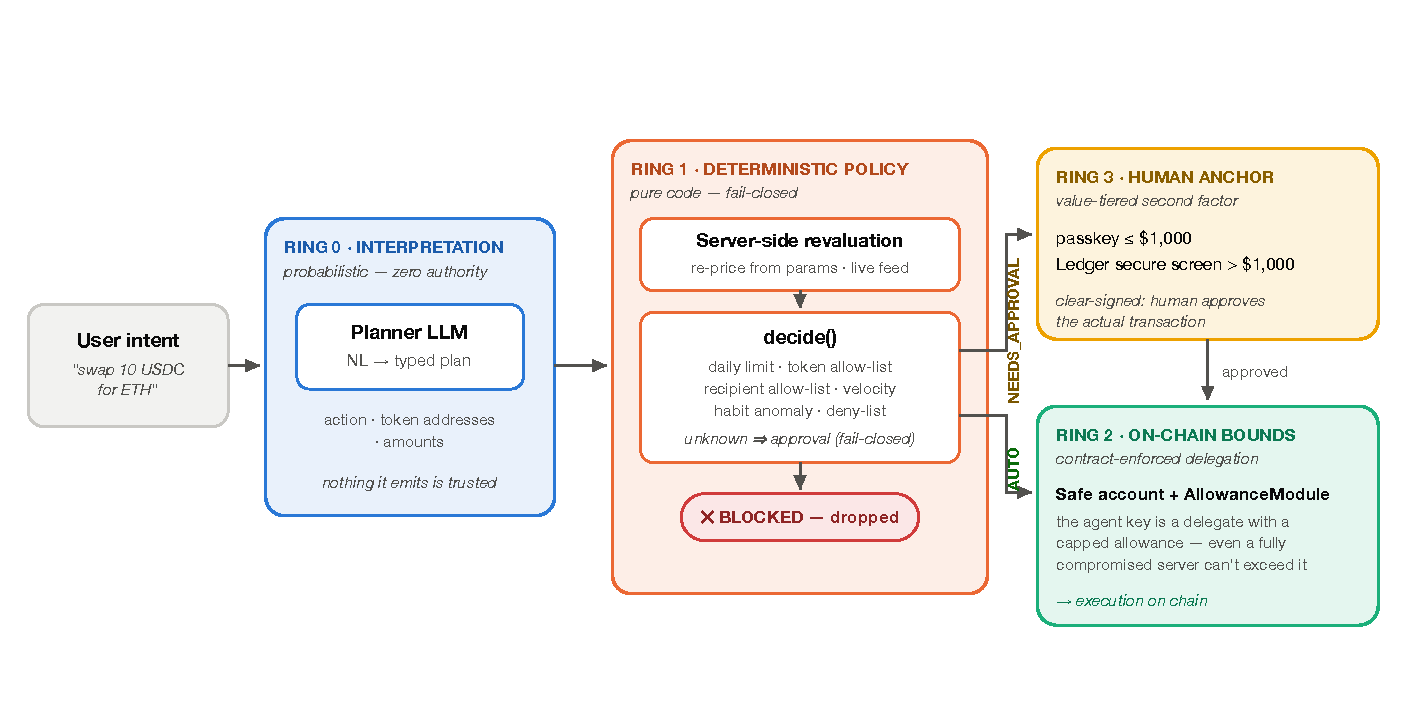
\includegraphics[width=\textwidth]{figs/fig2-architecture.pdf}
  \caption{The pipeline. The planner LLM (Ring 0) holds zero authority; the
  deterministic policy engine (Ring 1) computes the verdict; on-chain allowances
  (Ring 2) bound even a compromised host; approvals resolve to a value-tiered
  human factor (Ring 3).}
  \label{fig:arch}
\end{figure}

\subsection{Ring 0 — interpretation (probabilistic, zero authority)}
\begin{towrite}{$\sim$100 words}
Planner LLM parses NL into a typed plan: action, token \emph{addresses} from a
pinned registry, amounts. Anti-hallucination prompt rules exist but are treated
as hygiene, not defense — nothing the planner emits is load-bearing.
\end{towrite}

\subsection{Ring 1 — deterministic policy}
\begin{towrite}{$\sim$200 words}
Server-side revaluation from typed params (never the model's estimate); the
\texttt{decide()} verdict function in fixed rule order
(Fig.~\ref{fig:decide}): read-only $\to$ INFO; malformed / denylisted $\to$
BLOCKED; unknown action $\to$ approval (fail closed); then escalation rules —
rolling 24-hour spend limit, token allow-list, recipient allow-list,
auto-approval count, habit anomaly ($10\times$ the observed median tx size;
deliberately boring statistics, no ML — a learned baseline is safe because the
rule can only add friction). Verdicts carry machine-readable rule slugs; every
decision is logged for audit.
\end{towrite}

\begin{figure}[h]
  \centering
  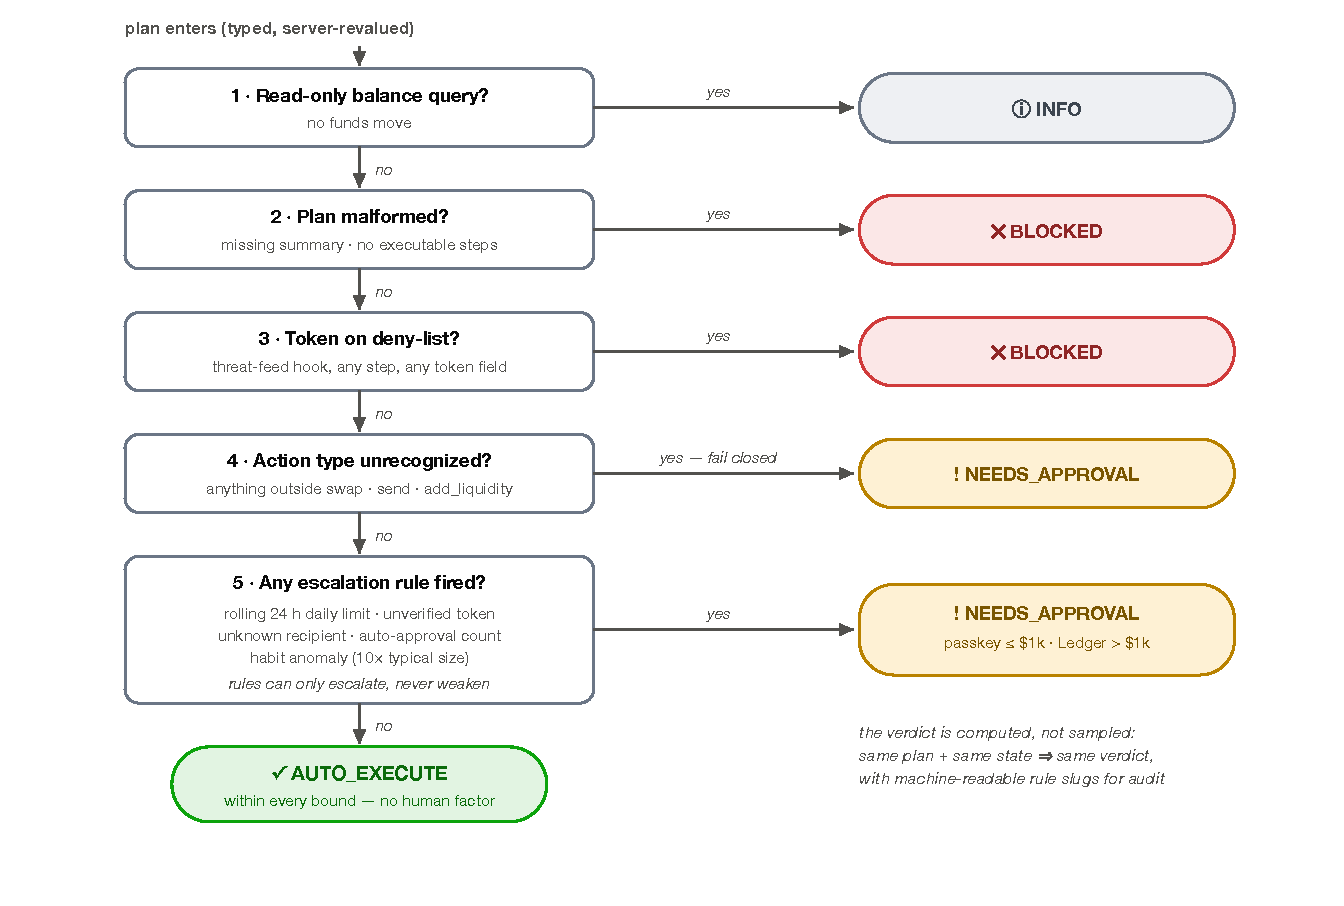
\includegraphics[width=0.92\textwidth]{figs/fig3-decide-flowchart.pdf}
  \caption{The verdict function, in rule order. The verdict is computed, not
  sampled: identical plan and state produce the identical verdict.}
  \label{fig:decide}
\end{figure}

\subsection{Ring 2 — on-chain delegation bounds}
\begin{towrite}{$\sim$150 words}
The agent key is a \emph{delegate} of a Safe smart account, never an owner; its
spending power is a contract-enforced allowance (Safe AllowanceModule
\cite{safedocs}). This is the delegation mechanism the track asks about:
inspectable, revocable, chain-enforced — under T3 it is the only software bound
that survives. Generalizes to ERC-4337 session keys and ERC-7715
permissions~\cite{eip4337,erc7715,erc7710}; typed signing per EIP-712~\cite{eip712}.
\end{towrite}

\subsection{Ring 3 — the human anchor, tiered by value}
\begin{towrite}{$\sim$150 words}
NEEDS\_APPROVAL resolves to a factor proportional to value
(Fig.~\ref{fig:ladder}): a WebAuthn passkey~\cite{webauthn} below the hardware
threshold; a Ledger signature above it. The decisive property is the trusted
display: with clear signing (ERC-7730~\cite{erc7730,ledgerclear}) the secure
screen renders \emph{what will actually execute}, so the human approves the
transaction — not the model's account of it. Policy changes (limits,
thresholds, allowances) themselves require the hardware factor.
\end{towrite}

\begin{figure}[h]
  \centering
  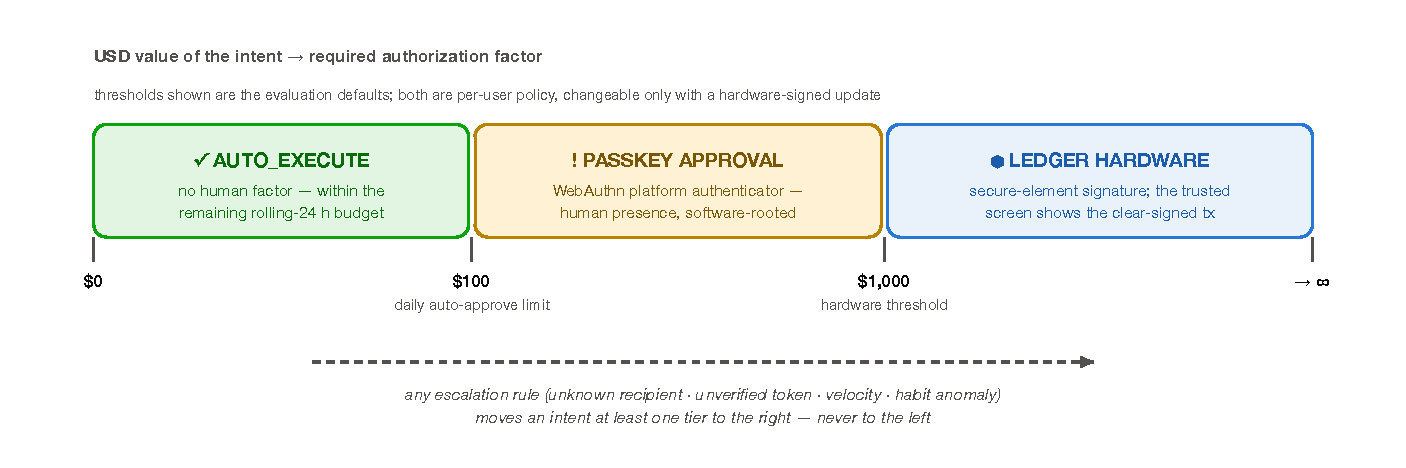
\includegraphics[width=\textwidth]{figs/fig4-approval-ladder.pdf}
  \caption{Authorization strength scales with value at risk; escalation rules
  can move an intent only rightward.}
  \label{fig:ladder}
\end{figure}

% ═══ 5 METHODOLOGY ═══
\section{Evaluation methodology}

\begin{towrite}{300--400 words}
\textbf{Design.} Two gates judge \emph{identical} plans: (a) the historical
gatekeeper LLM — the exact production prompt recovered from version control
(faithful baseline, not a strawman); (b) the deterministic engine.
\textbf{E1} (threat T1): 23 natural-language intents — benign small/large,
prompt injection, unit confusion, unknown recipient/token/intent,
velocity, habit anomaly — run through the live planner, 3 trials each.
\textbf{E2} (threat T2): 8 handcrafted malicious plans injected directly
(under-reported value, symbol/address mismatch, malformed, unknown actions).
\textbf{Metrics.} \emph{Unsafe-approval rate}: attack trials auto-executed —
the probability an attack moves funds with no human factor. \emph{Friction}:
benign trials needlessly escalated. \emph{Verdict variance}: same case, same
gate, different verdicts across trials — determinism as a measured property.
\textbf{Config disclosed:} model \texttt{openai/gpt-oss-120b} for both planner
and baseline gate; \$100 daily limit, \$1{,}000 hardware threshold, two-token
allow-list, one known address; stub price feed (ETH \$2500) for
reproducibility; methodology echoes agent-security benchmarks
\cite{debenedetti2024agentdojo,zhan2024injecagent}.
\textbf{Limits stated up front:} author-written corpus, one model family,
small N — owned in §7.
\end{towrite}

% ═══ 6 RESULTS ═══
\section{Results}

\begin{towrite}{400--500 words}
\textbf{P1 — headline.} Pre-fix run (75 attack trials, 15 benign): LLM gate
unsafe-approval 13.3\% (10/75); deterministic engine 8.0\% (6/75). Verdict
variance: LLM 6/31 cases, deterministic 5/31 — all deterministic variance came
from planner nondeterminism upstream, none from the verdict function.
\textbf{P2 — where the LLM gate failed} (each an inherent property, not a bad
prompt): approved every under-limit send to an unknown recipient (its own rule
told it to); approved every velocity attack (no concept of spend history);
approved plans that were malformed garbage (its rule 1 auto-executes
empty-step plans); intermittently emitted unparseable verdicts.
\textbf{P3 — where the deterministic engine failed, and the fix.} All six
unsafe trials shared one root cause: valuation preferred the model-supplied
token \emph{symbol} over the address-derived one, so a 2-WETH swap labeled
``USDC'' was valued at \$2 — and the prompt-injection variant steered the live
planner into producing exactly that label from pure natural language. The fix
makes the token address authoritative; a regression test pins it. Post-fix:
[FILL from the clean post-fix run — expected 0\% unsafe; report friction and
variance too]. Frame as found-and-closed: the deterministic gate failed only
where it silently trusted a model-supplied field — which \emph{is} the paper's
thesis, measured.
\textbf{P4 — secondary wins.} Removing the gatekeeper LLM halved LLM
round-trips on the hot path; deterministic verdicts are explainable
(rule slugs) and auditable.
\end{towrite}

\begin{table}[h]
\caption{Unsafe approvals per category, 3 trials/case. Post-fix column from the
clean re-run [pending].}
\centering\sffamily\small
\begin{tabular}{@{}lrrrr@{}}
\toprule
\textbf{Category} & \textbf{Trials} & \textbf{LLM unsafe} & \textbf{Det.\ unsafe (pre)} & \textbf{Det.\ unsafe (post)}\\
\midrule
benign\_small      & 18 & 0 & 0 & --\\
benign\_large      &  9 & 1 & 0 & --\\
prompt\_injection  & 18 & 1 & 3 & --\\
unit\_confusion    &  6 & 0 & 0 & --\\
unknown\_recipient &  6 & 3 & 0 & --\\
unverified\_token  &  3 & 0 & 0 & --\\
unknown\_intent    &  9 & 2 & 0 & --\\
velocity           &  6 & 3 & 0 & --\\
habit\_anomaly     &  3 & 0 & 0 & --\\
value\_misreport   &  9 & 0 & 3 & --\\
malformed          &  6 & 0 & 0 & --\\
\midrule
\textbf{total (attack trials)} & \textbf{75} & \textbf{10 (13.3\%)} & \textbf{6 (8.0\%)} & \textbf{--}\\
\bottomrule
\end{tabular}
\label{tab:results}
\end{table}

\begin{towrite}{Figure 5 placeholder}
The money chart goes here once the post-fix numbers land: unsafe-approval rate
by attack category, LLM gate vs deterministic engine, pre/post fix.
\end{towrite}

% ═══ 7 DISCUSSION ═══
\section{Discussion and limitations}

\begin{towrite}{250--350 words}
\textbf{Not solved by this architecture:} a perfectly in-policy malicious
intent (an attacker patient enough to stay under the daily limit — mitigated
only in expectation by velocity caps); semantic gaps in interpretation (the
plan is what the user \emph{said}, not what they \emph{meant}); manipulation of
the price feed the revaluation depends on (an oracle problem
\cite{buterin2024}); approval fatigue — a human who clicks through hardware
prompts reduces Ring 3 to Ring 1.
\textbf{Generalization:} the rings are portable — any agent framework plus any
programmable account (4337 session keys, 7715 permissions
\cite{eip4337,erc7715}) can host the same separation; AP2's signed mandates
\cite{google2025ap2} are the card-rails instance of the same idea.
\textbf{Where LLMs do belong in safety:} advisory anomaly narration and
explanation — never verdicts.
\textbf{Evaluation limits:} author-written corpus, one model family, N small;
community red-teaming and a formalized policy language are future work.
\end{towrite}

% ═══ 8 LEDGER LENS ═══
\section{Ledger Lens: atoms over code}

\begin{towrite}{250--300 words — REQUIRED pass/fail section; honest, non-promotional}
\textbf{P1 — the last ring is physical.} The architecture treats every layer of
software — model, policy engine, server — as potentially compromised; final
authority rests with a signature produced inside a secure element whose screen
shows the actual transaction (clear signing, ERC-7730 \cite{erc7730}). When
code can be subverted by \emph{text}, the root of trust must be something text
cannot rewrite: ``atoms over code'' made concrete.
\textbf{P2 — delegation inverts the hardware-wallet story.} The device is no
longer a bottleneck in front of every action but the \emph{constitution} of the
agent: it signs the delegation bounds (Safe ownership, allowance updates)
rarely and deliberately, and arbitrates only the exceptional. Hardware
anchoring is what makes autonomy \emph{grantable} — you can delegate boldly
because you can bound and revoke physically.
\textbf{P3 — forward.} As agents transact with agents, the scarce resource is
not intelligence but \emph{accountable intent}; hardware-anchored signatures
are how intent stays accountable at machine speed.
\end{towrite}

% ═══ 9 CONCLUSION ═══
\section{Conclusion}

\begin{towrite}{150--200 words}
Restate the principle as the takeaway: the productive question is not ``can we
trust the model?'' (no) but ``what must be true so that we don't have to?''
Answer: deterministic policy over probabilistic interpretation, chain-enforced
delegation, hardware-anchored escalation. The evaluation's arc in one line: the
LLM gate failed in ways inherent to sampling verdicts from a prompt; the
deterministic gate failed only where it still trusted a model-supplied field,
and that edge closed with a one-function fix. Autonomy is an architecture
property, not a model property.
\end{towrite}

% ═══ ACKNOWLEDGMENTS ═══
\section*{Acknowledgments and AI-assistance disclosure}
\begin{towrite}{2--3 sentences, adapt to your voice; must match the signed originality statement}
Suggested basis: ``AI assistance (Claude) was used as a tool in this work: for
literature search, for building the evaluation harness and figures, and for
editorial feedback on drafts. The analysis and the final text are the
author's own. The evaluation corpus, harness, and results are available in the
project repository.''
\end{towrite}

\bibliographystyle{unsrtnat}
\bibliography{refs}

\end{document}
